% !TEX program = lualatex
\RequirePackage{luatex85}
\PassOptionsToPackage{unicode}{hyperref}
\PassOptionsToPackage{naturalnames}{hyperref}
\documentclass{article}
\usepackage{geometry}
%\usepackage{fullpage}
\usepackage{parskip}
\usepackage{physics}
\usepackage{amsmath}
\usepackage{amssymb}
\usepackage{xcolor}
\usepackage[colorlinks,linkcolor=blue,citecolor=green]{hyperref}
\usepackage{array}
\usepackage{longtable}
\usepackage{multirow}
\usepackage{comment}
\usepackage{graphicx}
\usepackage{cite}
\usepackage{amsfonts}
\usepackage{bm}
\usepackage{slashed}
\usepackage{dsfont}
\usepackage{mathtools}
\usepackage[compat=1.1.0]{tikz-feynman}
\usepackage{simplewick}
\usepackage{mathrsfs}
\usepackage{xparse}
\usepackage{enumerate}
\usepackage{extarrows}

\newcommand{\calA}{\mathcal{A}}

\title{Note on Braaten's Paper}
\author{Yingsheng Huang}
\begin{document}
    \maketitle
    
    \section{Intro}
    Hamiltonian\cite{Braaten2008}: 
    \begin{align}
        \mathcal{H}=\sum_\sigma\frac{1}{2m}\nabla\psi_\sigma^{\dagger}\cdot\nabla\psi_\sigma^{(\Lambda)}+\frac{g(\Lambda)}{m}\psi^\dagger_1\psi^\dagger_2\psi_3\psi_4^{(\Lambda)}+\mathcal{V}
    \end{align}
    where the renormalized coupling 
    \begin{align}
        g(\Lambda)=\frac{4\pi a}{1-2a\Lambda/\pi}
    \end{align}

    \section{Amplitude}
    Consider: 
    \begin{align}
        i\calA=\mel{34}{\psi^\dagger\psi}{12}=
        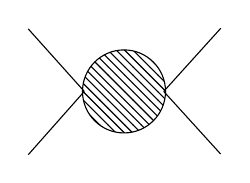
\begin{tikzpicture}[baseline=(o1.base)]
            \begin{feynman}
                \diagram[small,horizontal=o1 to o3]{
                    p1 -- o1 --[draw=none] o3 -- p3;
                    p2 -- o1 --[draw=none] o3 -- p4;
                };
                \node[blob, minimum size=30pt] at ($(o1)!0.5!(o3)$) (o2);
            \end{feynman}
        \end{tikzpicture}
    \end{align}
    Define $P=p_1+p_2=(E,\vb{0})$, and $E=p^2/m$. 
    The integral equation is 
    \begin{align}
        i\calA=-\frac{ig(\Lambda)}{m}\pqty{1+i\calA\int\bqty{\dd^4k}\frac{i}{k^0-\frac{\vb{k}^2}{2m}+i\epsilon}\frac{i}{k^0-p^0-\frac{\abs{\vb{k-p}}^2}{2m}+i\epsilon}}
    \end{align}
    The integral gives (redefine $\epsilon\rightarrow2m\epsilon$)
    \begin{align}
        \mathcal{I}=\frac{i m \left(-\Lambda +\sqrt{ -mE-i \epsilon } \tan ^{-1}\left(\frac{\Lambda }{\sqrt{ -mE-i \epsilon }}\right)\right)}{2 \pi ^2}
    \end{align}
    and 
    \begin{align}
        i\calA&=\frac{-1}{\mathcal{I}+\frac{m}{ig(\Lambda)}}=\frac{-1}{\frac{i m \sqrt{-mE -i \epsilon } \tan ^{-1}\left(\frac{\Lambda }{\sqrt{-mE -i \epsilon }}\right)}{2 \pi ^2}-\frac{i m}{4 \pi  a}}\\
        &\xlongequal{\Lambda\rightarrow\infty}\frac{4 i \pi/m  }{-1/a+ \sqrt{-mE -i \epsilon }}
    \end{align}

    {\bf Question: 
    Why only infinite bubbles in s-channel are considered? What about other channels?}

    \section{OPE}
    \subsection{l.h.s.}
    Take what we got in the last section as a new non-perturbative vertex, we only need to deal with tree diagram this way. First we have Figure~2(a) in Braaten's paper: 
    \begin{align}
        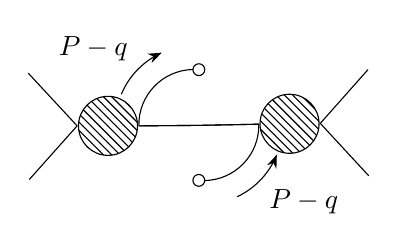
\begin{tikzpicture}[baseline=(o1.base)]
            \begin{feynman}
                \diagram[small,horizontal=o1 to o3]{
                    p1 -- o1 --[draw=none] o3 -- o35 -- o4 --[draw=none] o6 -- p3;
                    p2 -- o1 --[draw=none] o3 -- o35 -- o4 --[draw=none] o6 -- p4;
                };
                \node[empty dot] at ($(o3)!0.5!(o4)+(0,20pt)$) (ps1);
                \node[empty dot] at ($(o3)!0.5!(o4)+(0,-20pt)$) (ps2);
                \diagram*{
                    (o3) --[quarter left,momentum={[arrow shorten=0.25]\(P-q\)}] (ps1);
                    (ps2) --[quarter right,momentum'={[arrow shorten=0.25]\(P-q\)}] (o4);
                };
                \node[blob] at ($(o1)!0.5!(o3)$) (o2);
                \node[blob] at ($(o4)!0.5!(o6)$) (o5);
            \end{feynman}
        \end{tikzpicture}&=\mel{34}{\psi^\dagger\left(-\frac{\vb{r}}{2}\right)\psi\left(\frac{\vb{r}}{2}\right)}{12}\\
        &=\calA^2\int\frac{\dd^4q}{(2\pi)^4}\frac{i}{q^0-\frac{\vb{q}^2}{2m}+i\epsilon}\frac{i}{q^0-\frac{E-\vb{q}^2}{2m}+i\epsilon}\frac{i}{E-q^0-\frac{\vb{q}^2}{2m}+i\epsilon}e^{i\vb{q}\cdot\vb{r}}\\
        &=-\calA^2\int\frac{\dd^3\vb{q}}{(2\pi)^3}\frac{m^2e^{i\vb{q}\cdot\vb{r}}}{\pqty{\vb{q}^2-p^2-i\epsilon}^2}\\
        &=-\frac{i m^2\calA^2 e^{i p r}}{8 \pi  p}
    \end{align}

    \bibliography{../../QM-OPE/QM-OPE.bib}
    \bibliographystyle{unsrt}
\end{document}